\documentclass[tikz,border=20pt]{standalone}
\usepackage[T1]{fontenc}
\usepackage{tikz}
\usepackage{amsmath}
\usetikzlibrary{
  shapes.geometric,
  positioning,
  fit,
  backgrounds,
  shadows,
  arrows.meta,
  calc
}

\definecolor{layer1bg}{RGB}{240,248,255}
\definecolor{layer1border}{RGB}{70,130,180}
\definecolor{layer2bg}{RGB}{255,250,240}
\definecolor{layer2border}{RGB}{218,165,32}
\definecolor{layer3bg}{RGB}{240,255,240}
\definecolor{layer3border}{RGB}{60,179,113}

\begin{document}

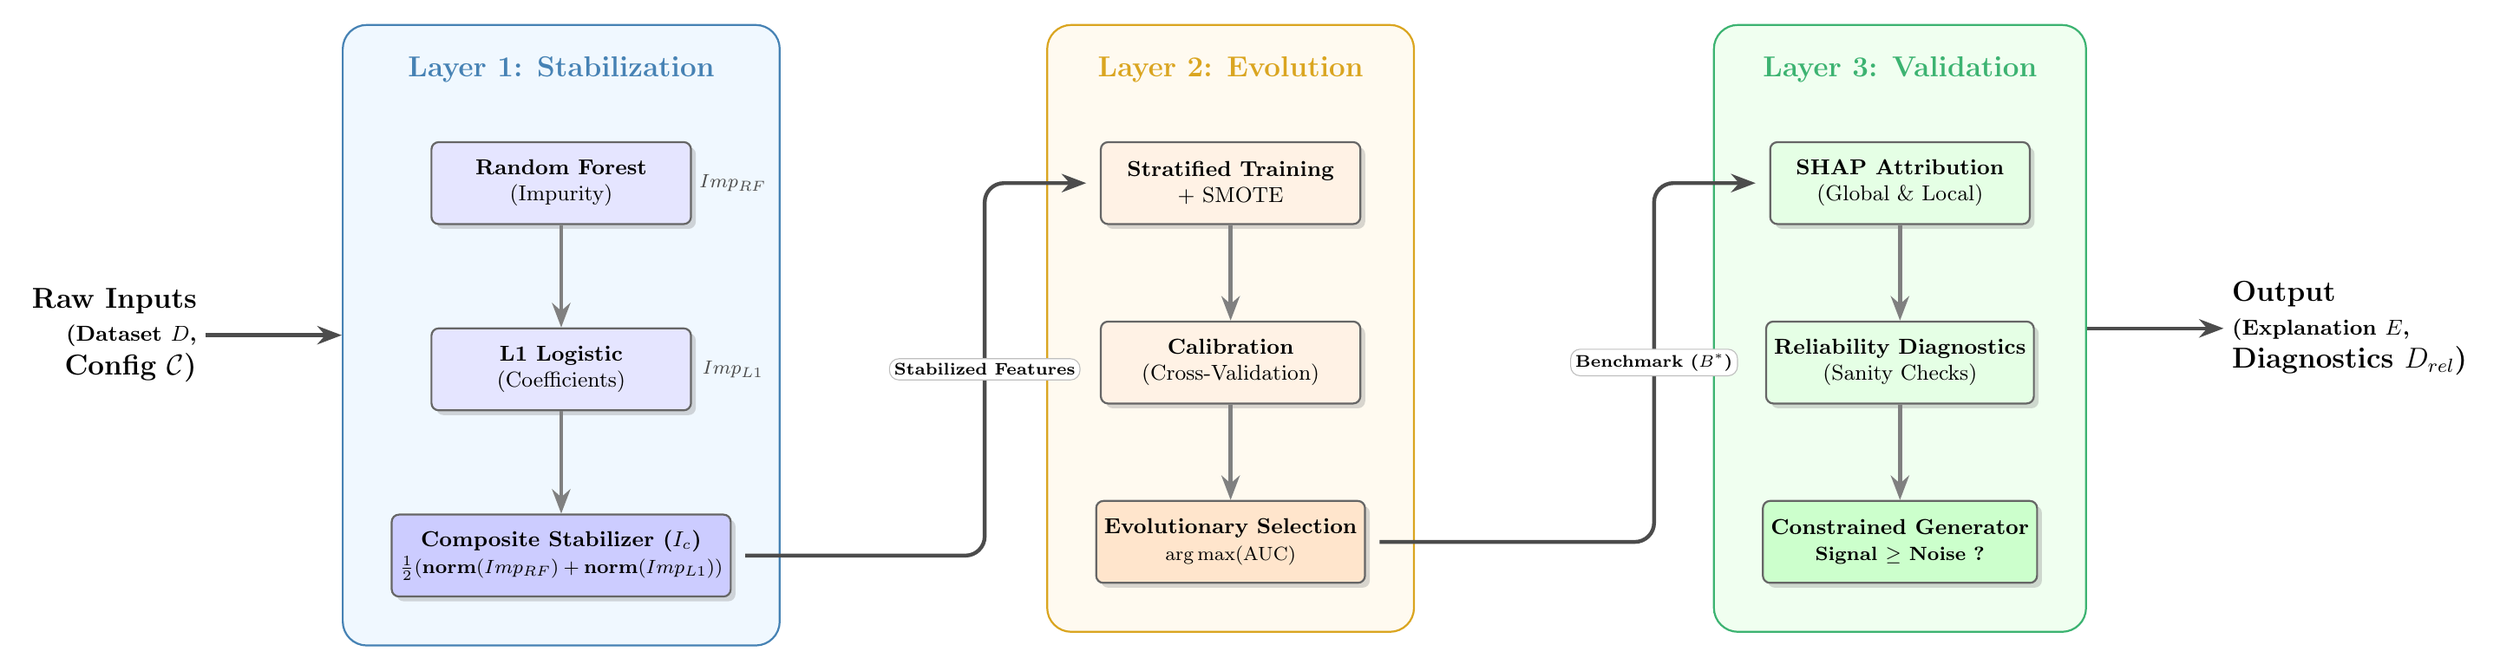
\begin{tikzpicture}[
  font=\sffamily,
  >=Stealth,
  component/.style={
    rectangle,
    rounded corners=3pt,
    draw=black!60,
    fill=white,
    thick,
    minimum height=1.2cm,
    minimum width=3.8cm,
    align=center,
    drop shadow={opacity=0.3,shadow xshift=2pt,shadow yshift=-2pt},
    font=\small\bfseries
  },
  logic/.style={
    draw=none,
    font=\footnotesize\itshape\color{black!70}
  },
  layer/.style={
    rectangle,
    rounded corners=10pt,
    draw,
    thick,
    inner sep=20pt
  },
  layerlabel/.style={
    font=\bfseries\large,
    anchor=north,
    yshift=-10pt
  },
  flow/.style={
    ->,
    ultra thick,
    black!70,
    rounded corners=8pt
  },
  arrowlabel/.style={
    fill=white,
    draw=gray!50,
    rounded corners,
    font=\scriptsize\bfseries,
    inner sep=2pt
  }
]

% ------------------------------------------------------------------
% Column anchors + routing spines (CRITICAL)
% ------------------------------------------------------------------
\coordinate (col1) at (0,0);
\coordinate (route12) at (6.2,0);
\coordinate (col2) at (9.8,0);
\coordinate (route23) at (16.0,0);
\coordinate (col3) at (19.6,0);

% ------------------------------------------------------------------
% Layer 1
% ------------------------------------------------------------------
\node[component, fill=blue!10] (rf) at ($(col1)+(0,2.8)$)
  {Random Forest\\ \normalfont (Impurity)};
\node[component, fill=blue!10, below=1.5cm of rf] (l1)
  {L1 Logistic\\ \normalfont (Coefficients)};
\node[component, fill=blue!20, below=1.5cm of l1] (composite)
  {Composite Stabilizer ($I_c$)\\
   \footnotesize $\tfrac12(\text{norm}(Imp_{RF})+\text{norm}(Imp_{L1}))$};

% FIXED label placement
\node[logic] at ($(rf.east)+(6mm,0)$) {$Imp_{RF}$};
\node[logic] at ($(l1.east)+(6mm,0)$) {$Imp_{L1}$};

\draw[flow,gray] (rf) -- (l1);
\draw[flow,gray] (l1) -- (composite);

% Reserve headroom for the layer title
\coordinate (layer1title) at ($(rf.north)+(0,10mm)$);

\begin{scope}[on background layer]
  \node[layer,draw=layer1border,fill=layer1bg,
        fit=(layer1title)(rf)(l1)(composite)] (layer1) {};
  \node[layerlabel,text=layer1border] at (layer1.north)
    {Layer 1: Stabilization};
\end{scope}

% ------------------------------------------------------------------
% Layer 2
% ------------------------------------------------------------------
\node[component, fill=orange!10] (training) at ($(col2)+(0,2.8)$)
  {Stratified Training\\ \normalfont + SMOTE};
\node[component, fill=orange!10, below=1.4cm of training] (calibration)
  {Calibration\\ \normalfont (Cross-Validation)};
\node[component, fill=orange!20, below=1.4cm of calibration] (selection)
  {Evolutionary Selection\\ \footnotesize $\arg\max(\mathrm{AUC})$};

\draw[flow,gray] (training) -- (calibration);
\draw[flow,gray] (calibration) -- (selection);

% Reserve headroom for title
\coordinate (layer2title) at ($(training.north)+(0,10mm)$);

\begin{scope}[on background layer]
  \node[layer,draw=layer2border,fill=layer2bg,
        fit=(layer2title)(training)(calibration)(selection)] (layer2) {};
  \node[layerlabel,text=layer2border] at (layer2.north)
    {Layer 2: Evolution};
\end{scope}


% ------------------------------------------------------------------
% Layer 3
% ------------------------------------------------------------------
\node[component, fill=green!10] (shap) at ($(col3)+(0,2.8)$)
  {SHAP Attribution\\ \normalfont (Global \& Local)};
\node[component, fill=green!10, below=1.4cm of shap] (diagnostics)
  {Reliability Diagnostics\\ \normalfont (Sanity Checks)};
\node[component, fill=green!20, below=1.4cm of diagnostics] (generator)
  {Constrained Generator\\ \footnotesize Signal $\ge$ Noise ?};

\draw[flow,gray] (shap) -- (diagnostics);
\draw[flow,gray] (diagnostics) -- (generator);

% Reserve headroom for title
\coordinate (layer3title) at ($(shap.north)+(0,10mm)$);

\begin{scope}[on background layer]
  \node[layer,draw=layer3border,fill=layer3bg,
        fit=(layer3title)(shap)(diagnostics)(generator)] (layer3) {};
  \node[layerlabel,text=layer3border] at (layer3.north)
    {Layer 3: Validation};
\end{scope}


% ------------------------------------------------------------------
% Inter-layer routing (NO overlaps possible)
% ------------------------------------------------------------------
\coordinate (port1) at ($(composite.east)+(0.2,0)$);
\coordinate (port2) at ($(training.west)+(-0.2,0)$);

\draw[flow] (port1) -- (route12 |- port1) -- (route12 |- port2) -- (port2);
\node[arrowlabel] at ($(route12 |- port1)!0.5!(route12 |- port2)$)
  {Stabilized Features};

\coordinate (port3) at ($(selection.east)+(0.2,0)$);
\coordinate (port4) at ($(shap.west)+(-0.2,0)$);

\draw[flow] (port3) -- (route23 |- port3) -- (route23 |- port4) -- (port4);
\node[arrowlabel] at ($(route23 |- port3)!0.5!(route23 |- port4)$)
  {Benchmark ($B^*$)};

% ------------------------------------------------------------------
% Global input / output
% ------------------------------------------------------------------
\node[left=2.0cm of layer1,align=right,font=\bfseries\large] (inputs)
  {Raw Inputs\\ \small (Dataset $D$,\\ Config $\mathcal C$)};
\draw[flow] (inputs) -- (layer1.west);

\node[right=2.0cm of layer3,align=left,font=\bfseries\large] (outputs)
  {Output\\ \small (Explanation $E$,\\ Diagnostics $D_{rel}$)};
\draw[flow] (layer3.east) -- (outputs);

\end{tikzpicture}
\end{document}
